% ----------------------------  START --------------------------- 
\documentclass[../main]{subfiles} % main refers to main.tex
\graphicspath{{\subfix{../Illustrations}}}
\begin{document}
\addto\extrasfrench{\protected\edef:{\unexpanded\expandafter{:}}}
\selectlanguage{french}
% --------------------------------------------------------------- 

\begin{figure}[ht]
    \centering
    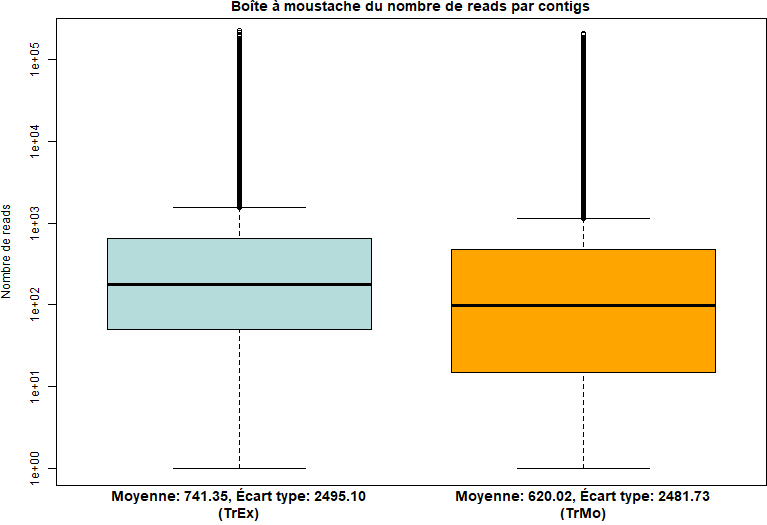
\includegraphics[width=0.9\textwidth]{../Illustrations/boxplotTr.png}
    \caption{Boite à moustache du nombre de \reads\,par \contigs. Les données relatives à \BamTrEx\,sont a gauche tandis que les données relatives a \BamTrMo\, sont à droite. Seuls les \contigs\,ayant au moins 1 \reads\,ont été pris en compte. Figure générée sur \gls{R} puis modifiée avec \gls{gimp} pour fusionner les deux boites à moustaches sur le même graphique.}
    \label{fig:BoxPlotContigs}
\end{figure}


% --------------------------------------------------------------- 
\end{document}
% ----------------------------  END --------------------------- 
